\chapter[Produtos, Atividades e Cronograma]{Produtos, Atividades e Cronograma}

\section{Resumo da proposta}

Este trabalho pretende analisar a verificação da qualidade no desenvolvimento de jogos eletrônicos a partir da analise estática de código e do desenvolvimento de testes unitários tendo em vista a definição do grau de dificuldade e efetividade do controle de qualidade de código no processo de produção de jogos eletrônicos.
Determinar não como testar, que segundo \citeonline{artoftest} testar é o processo de executar um programa com a intenção de encontrar erros, mas principalmente o que deve ser testado, dado que no contexto as mudanças acontecem de forma acentuada uma cobertura total aumentaria o trabalho de testar tais mudanças.

\section{Estrutura Analítica do Projeto}

A figura a seguir mostra a estrutura analítica do projeto. O projeto foi dividido em 3 fases: Iniciação, cujo objetivo é obter a viabilidade e a construir o referencial teórico do projeto; Construção, cujo objetivo é realizar de fato as atividades de testes e análise estática; e Transição, cujo objetivo é entregar a integração contínua e finalizar o projeto.
\begin{figure}[h]
 \centering
 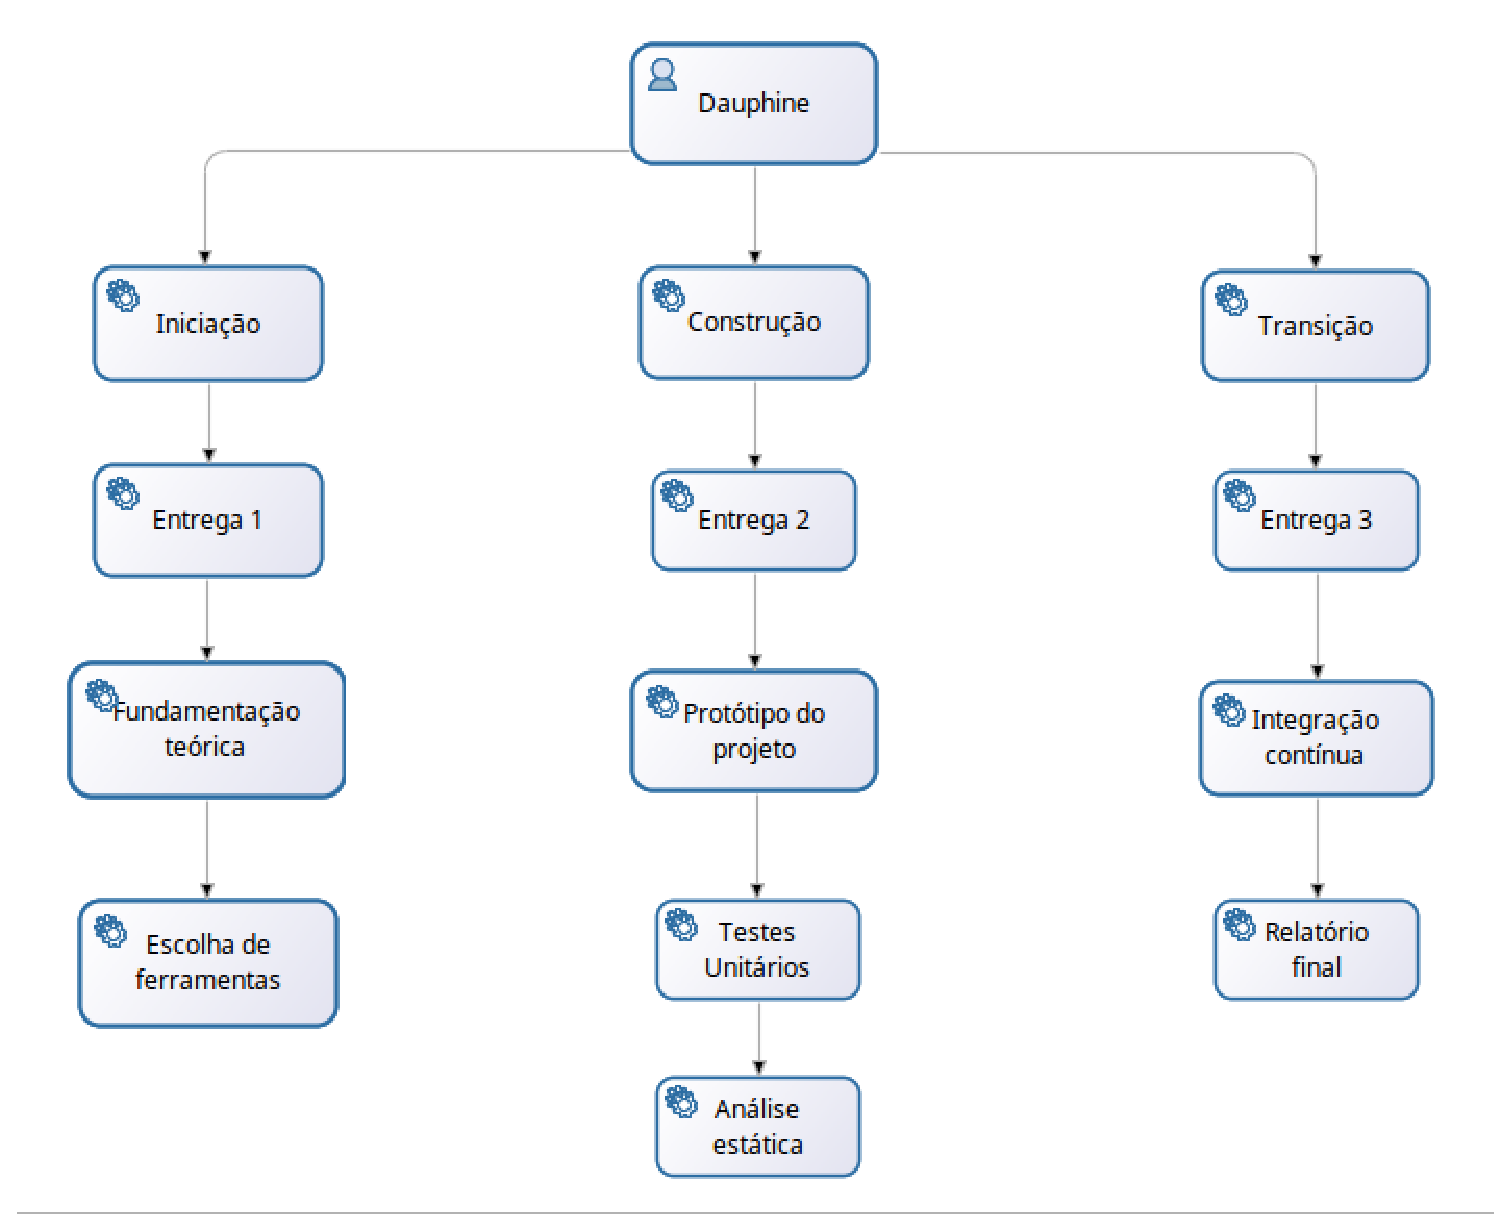
\includegraphics[scale=0.4]{figuras/eap.eps}
 \caption{Estrutura Analítica do Projeto}
\end{figure}

\section{Lista de Software}

\begin{itemize}
\item{Linguagem de programação:} \textbf{C++}
Sua alta performance e qualidade, segue na liderança disparada em produção de jogos.
\item{Compilador:} \textbf{GNU Compiler Collection (gcc)}
Confiável e com bom suporte ao padrão C++11.
\item{Controle de versão de código e documentação:} \textbf{Git (GitHub)}
Na liderança popular entre os forges de Git por sua qualidade e poder de socialização. O repositório pode ser acessado neste \href{https://github.com/CaioIcy/Dauphine}{link}.
\item{Editor de texto:} \textbf{Sublime Text}
Preferido pelos desenvolvedores da equipe.
\item{Gerador de documentação:} \textbf{Doxygen}
Um gerador de documentação excelente, e compátível com C++. A documentação do código será hospedada \textit{online} em uma \textit{GitHub page}.
\item{Ferramenta de Análise Estática:} \textbf{Analizo}
Uma ferramenta que extrai diversas métricas de código-fonte para diversas linguagens, inclusive C++.
\item{Ferramenta de Integração Contínua:} \textbf{Travis CI}
Uma ferramenta online e gratuita de integração contínua com suporte para muitas linguagens de programação.
\item{Ferramenta de Testes Unitários:} \textbf{Google Test}
Preferido pelos desenvolvedores da equipe
\item{Sistema operacional de desenvolvimento:} \textbf{Linux Debian Based}
\end{itemize}

\section{Cronograma de Atividades}

O cronograma deste trabalho se encontra neste \href{https://trello.com/b/9Y8n9q5X/vv-dauphine}{link}
